% !TeX encoding = UTF-8
% !TeX root = ../main.tex

%% PPOM-Attack 组会汇报（10 分钟）
%% 数据来源：IEEE TIFS 2026, DOI 10.1109/TIFS.2026.3666853
%% 所有数字取自论文正文叙述与 Table III / IV / V / VII / IX / XI

\section{问题}

\begin{frame}{一页看懂}
  \vspace{-3.6em}
  \begin{columns}[T]
    \column{.32\textwidth}
    \begin{block}{问题}
      黑盒人脸识别攻击中，替代模型\alert{不能}准确逼近目标模型，
      迁移性假设失效，攻击成功率与画质同时下降。
    \end{block}

    \column{.32\textwidth}
    \begin{block}{做法}
      不用替代模型，直接拿目标模型反馈；
      PPO 智能体\textbf{选区域}，再对该区域做\textbf{整体亮度偏移}。
    \end{block}

    \column{.32\textwidth}
    \begin{block}{结果}
      ASR 平均 \alert{+21.7\%}（LFW）/ +22.9\%（CelebA-HQ）；
      LPIPS \alert{0.0062}；平均查询 \alert{2007} 次。
    \end{block}
  \end{columns}

  \vspace{1.2em}
  \begin{center}
    \small 一句话：把扰动单元从「单像素」换成「整块亮度」，攻击从 1\% 变成 100\%。
  \end{center}
\end{frame}

\begin{frame}{背景：两条路线，同一个隐含假设}
  \vspace{-2pt}
  \begin{columns}[T]
    \column{.56\textwidth}
    \small
    \begin{itemize}
      \item \textbf{替代模型 + 梯度}：PGD、TI-RDIM、TIP-IM、Sibling-Attack、DPA
      \item \textbf{替代模型 + 生成模型}：Adv-Makeup、AMT-GAN、Clip2Protect、AdvDiffusion
    \end{itemize}

    \vspace{-0.3em}
    \begin{alertblock}{共同前提}
      \footnotesize
      扰动必须活在\textbf{像素级、连续、可微}的空间里；
      替代模型的决策边界要与目标模型「足够接近」。
    \end{alertblock}

    \vspace{-0.3em}
    \begin{itemize}
      \item 架构（ResNet / DenseNet / VGGFace）、训练数据不同 →
            \alert{替代模型与目标模型存在系统性偏差}
      \item 于是在替代模型上打得好，\textbf{在目标模型上大幅掉点}
    \end{itemize}

    \column{.42\textwidth}
    \begin{minipage}{\linewidth}
      \setlength{\parindent}{0pt}
      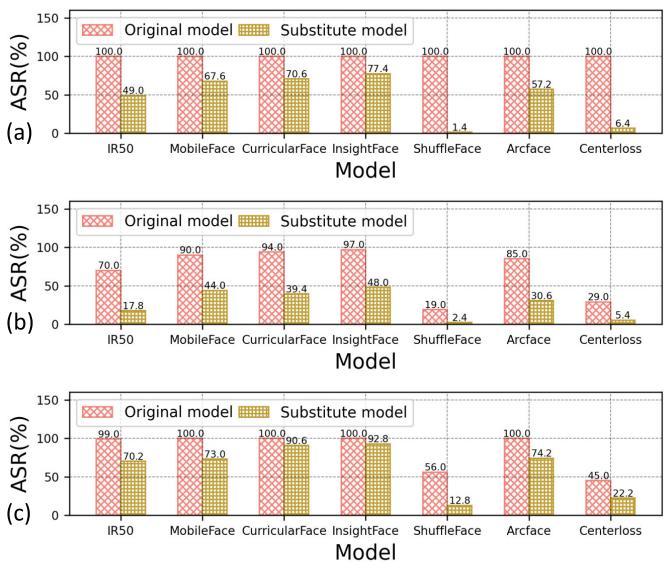
\includegraphics[width=\linewidth]{ppom/fig1-substitute-gap.jpg}

      {\footnotesize
      \textbf{Fig.~1}\quad 同一批对抗人脸在替代 / 目标模型上的 ASR：
      替代模型接近饱和，目标模型明显塌陷——本文要消掉的误差项。\par}
    \end{minipage}
  \end{columns}
\end{frame}

\begin{frame}{威胁模型：把「不知道」写死}
  \vspace{-3.6em}
  \begin{columns}[T]
    \column{.5\textwidth}
    \begin{block}{攻击者目标}
      让目标 FR 模型（\textbf{含对抗训练防御的模型}）
      把对抗人脸识别为指定身份，且视觉上不明显。
    \end{block}
    \vspace{0.6em}
    \begin{block}{背景知识}
      对目标模型\textbf{零知识}：架构、参数、配置、训练数据一概不知，
      因此也拿不到梯度。
    \end{block}

    \column{.46\textwidth}
    \begin{block}{能力与约束}
      \begin{itemize}
        \item 能收集目标身份的人脸图（社交平台即可）
        \item 能反复查询，但只返回\textbf{识别结果 + 置信度}
        \item 查询预算 \alert{10\,000} 次
        \item 扰动受 $\ell_\infty \le \epsilon$ 约束
      \end{itemize}
    \end{block}
    \vspace{0.3em}
    \small 形式上：$\min_{x^a} D\big(f(x^a), f(x^t)\big)$，
    s.t. $\lVert x^a - x^o \rVert_\infty \le \epsilon$。
  \end{columns}
\end{frame}

\section{方法}

\begin{frame}{核心思路：换掉扰动的「表示形式」}
  \begin{center}
    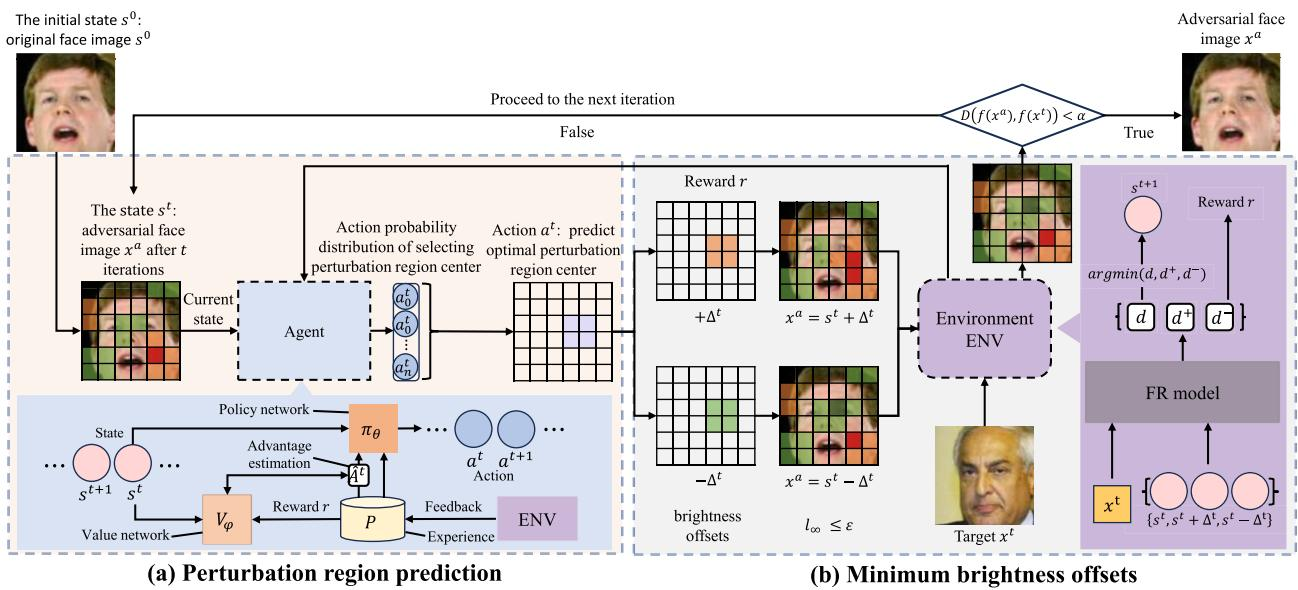
\includegraphics[width=.72\textwidth]{ppom/fig3-arch.jpg}
  \end{center}
  \vspace{-0.8em}
  \small
  两级层次结构：\textbf{区域级}动作（智能体决定扰动哪一块）
  $\rightarrow$ \textbf{像素级}修改（块内整体加减亮度）。
  \begin{itemize}
    \item 不做梯度反传，不做生成模型，只做「选区域 + 试符号」
    \item 扰动被限制在\textbf{空间连贯}的方块内，天然抑制高频噪声
  \end{itemize}
\end{frame}

\begin{frame}{模块一：PPO 智能体预测扰动区域}
  把加扰动建模成马尔可夫决策过程：
  \begin{itemize}
    \item \textbf{状态} $s^t$：当前对抗图（初值为原图 $x^o$）
    \item \textbf{动作} $a^t$：区域中心，$a^t \in \{1,\dots,w^2\}$；
          区域边长 $\sqrt{\rho w^2}$（默认 $\rho = 0.02$）
    \item \textbf{网络}：2 层卷积 + 3 层全连接，策略头输出全图区域概率，价值头输出 $V(s^t)$
    \item \textbf{奖励}：$r^t = \beta(\alpha - d^{t+1}) + (d^t - d^{t+1})$，$\beta=0.001$，$\alpha=15$
  \end{itemize}

  \vspace{0.4em}
  \begin{block}{为什么是 PPO，而不是 DQN / TD3}
    \begin{itemize}
      \item 动作空间 $w^2$ 极大，逐个估 $Q(s,a)$ 或取 $\arg\max$ 不可行
      \item 每加一次扰动，状态分布立刻漂移 → 回放池里的旧样本很快失配，
            off-policy 的 $Q$ 估计在有限查询预算下不稳定
      \item 因此选 on-policy 的策略梯度：裁剪 $\eta=0.2$、$\gamma=0.99$、$\lambda=0.95$，
            每 $T=10$ 步更新一次，配熵正则与梯度裁剪 0.5
    \end{itemize}
  \end{block}
\end{frame}

\begin{frame}{模块二：最小亮度偏移}
  \begin{columns}[T]
    \column{.5\textwidth}
    对选定区域 $R(a^t)$，构造两个候选：
    \begin{itemize}
      \item 全 $+1$ 矩阵 $+\Delta^t$（整体调亮）
      \item 全 $-1$ 矩阵 $-\Delta^t$（整体调暗）
    \end{itemize}
    \vspace{0.2em}
    \footnotesize
    分别查询目标模型、算与目标身份的嵌入距离：
    \[
      \begin{aligned}
        d^{t+1} = \min\big\{ & D(f(s^t{+}\Delta^t), f(x^t)), \\
                             & D(f(s^t{-}\Delta^t), f(x^t)), \\
                             & D(f(s^t), f(x^t)) \big\}
      \end{aligned}
    \]
    \normalsize 取最小者；\textbf{若没有改进则拒绝这一步}。

    \column{.46\textwidth}
    \begin{block}{两个工程细节}
      \begin{itemize}
        \item 每步只发 \alert{2 次查询}（$+\Delta$ 与 $-\Delta$），
              这就是查询效率的来源
        \item 像素裁剪到
              $[\max(0, x^o{-}\epsilon),\, \min(x^o{+}\epsilon, 255)]$，
              硬保证 $\ell_\infty$ 约束
      \end{itemize}
    \end{block}
    \vspace{0.3em}
    \small
    单步偏移量：常规 $\pm 1$；攻商用 API 时用 $\pm 5$，
    因为接口返回的反馈信号更粗，需要更强的单步扰动才能形成可分辨的奖励差。
  \end{columns}
\end{frame}

\section{实验}

\begin{frame}{关键消融：1\% $\rightarrow$ 100\%}

  \begin{center}
    \scriptsize
    \begin{tabular}{lcccc}
      \toprule
      LFW 数据集 & IR50 & MobileFace & InsightFace & ArcFace \\
      \midrule
      全采样 + 分块亮度（无智能体） & 98.0 & 98.0 & 100.0 & 94.6 \\
      智能体 + \alert{逐像素偏移}     & \alert{1.0} & \alert{1.0} & \alert{1.0} & \alert{1.0} \\
      智能体 + 分块亮度（本文）        & 100.0 & 100.0 & 100.0 & 94.6 \\
      \midrule
      平均查询数（全采样 / 本文）      & 13122 / 2007 & 11906 / 1638 & 10373 / 1252 & 11358 / 1635 \\
      \bottomrule
    \end{tabular}
  \end{center}

  \vspace{-0.2em}
  \begin{columns}[T]
    \column{.48\textwidth}
    \begin{alertblock}{同一套策略、同一查询预算}
      \scriptsize
      只把扰动单元从\textbf{单个像素}换成\textbf{整块均匀亮度}，
      成功率从 1\% 跳到接近 100\%。
    \end{alertblock}

    \column{.48\textwidth}
    \begin{exampleblock}{但要看清楚两件事}
      \scriptsize
      \begin{itemize}
        \item 逐像素组 PSNR 高达 \textbf{57.1}（画质“更好”），ASR 却只有 1\%
              —— \textbf{攻击失败时画质指标没有意义}
        \item 智能体的增益主要在\textbf{查询数}（13122$\rightarrow$2007），
              而非成功率（98.0$\rightarrow$100.0）
      \end{itemize}
    \end{exampleblock}
  \end{columns}
\end{frame}

\begin{frame}{主结果：成功率、画质、查询数}
  \begin{columns}[T]
    \column{.55\textwidth}
    \small
    \begin{tabular}{lccc}
      \toprule
      方法 & ASR & LPIPS$\downarrow$ & PSNR$\uparrow$ \\
      \midrule
      PGD          & 64.0 & 0.0507 & 32.46 \\
      TI-RDIM      & 42.6 & 0.1838 & 24.35 \\
      Clip2Protect & 71.4 & 0.3425 & 12.55 \\
      Sibling-Attack & 89.4 & 0.1720 & 25.48 \\
      AdvDiffusion & 62.0 & 0.3053 & 14.30 \\
      DPA          & 41.6 & 0.1164 & 29.76 \\
      \midrule
      \textbf{PPOM-Attack} & \textbf{100.0} & \textbf{0.0062} & \textbf{33.25} \\
      \bottomrule
    \end{tabular}
    \vspace{0.2em}
    \footnotesize LFW / IR50 一列；$\ell_2$ 范数 1126，与 PGD 的 1193 同量级。
    \column{.42\textwidth}
    \begin{block}{和查询式方法比（Table IV）}
      \small
      查询上限统一 10k：
      \begin{itemize}
        \item 本文平均 \alert{2007} 次
        \item Sparse-RS 2874、BruSLeAttack 2775
        \item GSBAK 6438
        \item Evolution / CGBA / DevoPatch 直接打满 10000
      \end{itemize}
    \end{block}
    \vspace{-0.4em}
    \footnotesize
    LPIPS 低一个数量级：分块均匀亮度几乎不引入高频纹理，看起来只是「某处亮/暗了一点」。
  \end{columns}
\end{frame}

\begin{frame}{打穿对抗训练，以及商用 API}
  \begin{columns}[T]
    \column{.5\textwidth}
    \small
    \begin{tabular}{lcc}
      \toprule
      ASR(\%) & PGD-AT & TRADES \\
      \midrule
      Sibling-Attack & 2.8 & 4.6 \\
      Clip2Protect   & 4.8 & 22.0 \\
      AdvDiffusion   & 3.8 & 12.6 \\
      \midrule
      \textbf{PPOM-Attack} & \textbf{20.6} & \textbf{54.8} \\
      \bottomrule
    \end{tabular}
    \vspace{0.3em}

    \footnotesize LFW 一列；CelebA-HQ 上为 36.8 / 92.4。
    TRADES 上差距最大：\textbf{54.8 vs 22.0}。

    \vspace{0.6em}
    \begin{block}{为什么能打穿}
      \footnotesize
      对抗训练让模型在\textbf{梯度方向}上变平滑；\\
      而「整块亮度偏移」走的是低维、离散、\textbf{与梯度不对齐}的空间。
    \end{block}

    \column{.46\textwidth}
    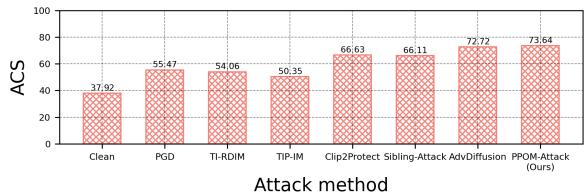
\includegraphics[width=\textwidth]{ppom/fig5-facepp-acs.jpg}
    \vspace{-0.2em}
    \footnotesize
    \textbf{Fig.~5}：Face++ 返回的平均置信度（越高越好）。
    商用接口上同样领先；用 MTCNN 提人脸区域加掩码，
    保证智能体不会选到非人脸区域。
  \end{columns}
\end{frame}

\section{讨论}

\begin{frame}{局限}
  \vspace{-3.6em}
  \begin{columns}[T]
    \column{.49\textwidth}
    \begin{block}{论文自己承认的}
      \small
      \begin{itemize}
        \item \textbf{Centerloss 只有 67.0}（LFW）/ 70.4（CelebA-HQ）。
              作者归因于骨干差异：它是 VGGFace，其余是 ResNet
        \item ShuffleFace 在 CelebA-HQ 只有 \textbf{64.8}（DenseNet 骨干）
        \item 反馈过于稀疏时效率下降；查询次数多，\textbf{可能被异常检测抓}
      \end{itemize}
    \end{block}

    \column{.47\textwidth}
    \begin{alertblock}{可以追问的要点}
      \small
      \begin{itemize}
        \item $\rho$ 与单步 $\pm\Delta$ 都是手工定的；
              换数据集还得重调（Face++ 就得从 $\pm1$ 改 $\pm5$）
        \item 严格说这\textbf{不是「生成」对抗样本}：没有生成模型、没有梯度，
              是离散搜索式扰动优化
      \end{itemize}
    \end{alertblock}
  \end{columns}
\end{frame}
